\chapter[Introduction]{Introduction}
\chaptermark{Introduction}
\label{chap:introduction}
% TODO: remove
And Schmidhuber said, Let there be backpropagation, and there was backpropagation.
\minitoc
\section{Foreword}
\label{in:sec:foreword}
This thesis investigates data driven endoscopic camera motion automation by means of a robot and therefore falls into the realm of robot assisted surgery (RAS). It aims to find novel ways that support clinical staff in their daily work by elevating them of unfulfilling tasks and it takes enhanced patient care as its core guiding principle.

In RAS, it is commonly acknowledged that automation will proceed stepwise. From no autonomy to full automation, these steps are often categorized into six stages \cite{zhang2017automation, fosch2021human}:
\begin{enumerate}
    \item No autonomy: Surgeon is in full charge of the robot
    \item Robot assistance: Robot constrains motion and corrects surgeon  
    \item Task autonomy: Robot executes specific tasks autonomously under human supervision
    \item Conditional autonomy: Robot plans and executes tasks under human approval
    \item High autonomy: As conditional autonomy without approval but human intervention
    \item Full automation: Robot performs an entire surgery autonomously
\end{enumerate}
This work explores level five, high autonomy, which would require approval-free endoscopic camera motion execution with the possibility of human intervention. Although some works \cite{battaglia2021rethinking} argue that the focus should not lie on automation, rather enhancement, we adopt a futuristic sentiment and are in alignment with \cite{kitaguchi2022artificial}, where the authors explain why camera motion automation will likely be achieved first. This futuristic notion follows previous surgical revolutions, from the advancement of open surgery to minimally invasive surgery (MIS), and the success of the da Vinci\textsuperscript{\textregistered} surgical robot in robot assisted minimally invasive surgery (RMIS), see also \figref{in:fig:camera_motion_automation} and \figref{in:fig:robotic_vs_laparoscopic_vs_open}.

The ever evolving field of surgery has repeatedly demonstrated gradual acceptance of new technology \cite{attanasio2021autonomoy}, and we argue that automation is no exception. The growth of RMIS can clearly be considered an enabling factor for full automation, see also \figref{in:fig:camera_motion_automation}.
\begin{figure}
    \centering
    \includegraphics[width=0.8\textwidth]{introduction/fig/24_02_13_surgical_revolution.pdf}
    \caption{The gradual introduction of novel technology into the surgical field, one enabling the next. Endoscopic camera motion automation is likely to appear first towards full automation. Refers to \secref{in:sec:foreword}.}
    \label{in:fig:camera_motion_automation}
\end{figure}
When compared to other domains, such as autonomous driving, service and household robots, where robots already exert a significant amount autonomy that far exceeds RMIS, it becomes obvious that these advances will ultimately make their way into the operating theater as well. This is because the medical field usually adopts novel technology in the order of tens of years later due to regulatory hurdles and cost. However, there might even be a future where RMIS will not only adopt full automation from other domains but make significant contributions to general machine intelligence. Others \cite{lecun2022path} have argued that machines will need to interact with the real world in order to become truly intelligent and, arguably, RMIS has grown to be the most advanced physical human-robot interaction (pHRI) domain with thousands of deployed robots.

As we dive deeper into level five autonomy endoscopic camera motion automation, the introductory chapter will provide a solid clinical background for laparoscopy, a sub-domain of endoscopy, in \secref{in:sec:laparoscopy}, including an in-depth explanation of laparoscopic cholecystectomy (minimally invasive gallbladder removal). This is because laparoscopic cholecystectomy is performed in high volumes and can be considered a relatively simple procedure. It serves as the perfect test-bed for the methods that will be derived as part of this thesis. Next, we explain the rise of robot assisted laparoscopy in \secref{in:sec:robot_assisted_laparoscopy} and the potentials of automation that evolve with it. We highlight different commercial systems, their limitations, and propose solutions.

\secref{in:sec:spatial_awareness}

\secref{in:sec:camera_motion_automation}

follow a hypothesis-based approach that will be rigorously tested
\secref{in:sec:hypothesis_one}
\secref{in:sec:hypothesis_two}

\begin{figure}
    \centering
    \includegraphics[width=0.7\textwidth]{introduction/img/robotic_since_introduction.png}
    \caption{Shown is the increase of minimally invasive laparoscopy over open approaches from 2012 to 2018. Indicated as year zero is the introduction of robotic laparoscopy, which increased from $1.8\%$ in 2012 to $15.1\%$ in 2018. For inguinal hernia repair, an even greater increase in robotic surgery was identified from $0.7\%$ to $28.8\%$. A total of $169.404$ cases were investigated. Figure and data provided with courtesy by \cite{sheetz2020trends}. Refers to \secref{in:sec:foreword}.}
    \label{in:fig:robotic_vs_laparoscopic_vs_open}
\end{figure}

\section{Laparoscopy}
\label{in:sec:laparoscopy}
Endoscopy refers to the observation of internal parts by means of an endoscope \cite{oedendoscopy}. The word endoscopy derives from the Greek by combining the prefix "endo" meaning "within" and the verb "skopein", "to view or observe" \cite{majumdar1993short}. In the surgical context, endoscopy refers to a MIS with the goal to observe within the body. Endoscopy inside the abdominal (belly) or pelvic (hip) cavity is called laparoscopy. During laparoscopy, a laparoscope is inserted through small incisions for diagnostic or interventional purposes, see \figref{in:fig:laparoscopy}.

\begin{figure}
    \centering
    \includegraphics[width=0.7\textwidth]{introduction/img/laparoscopy-min.png}
    \caption{Illustration of a laparoscopic procedure. The laparoscope is inserted through a small incision in the patient's abdominal wall and provides a view of the surgical scene. To provide space, carbon dioxide ($\text{CO}_2$) is injected through a needle into the abdomen. Image provided with courtesy by \cite{blausen2014laparoscopy}. Refers to \secref{in:sec:laparoscopy}.}
    \label{in:fig:laparoscopy}
\end{figure}

Compared to open surgery, laparoscopy leads to significantly faster interventions ($57.19\pm10.13\,\text{min}$ vs. $85.10\pm15.18\,\text{min}$), less bleeding complications ($2\%$ vs $7\%$ of interventions), shorter hospital stays ($2.1\pm1.1\,\text{days}$ vs $4.4\pm2.1\,\text{days}$), less infections, and less post-operative pain \cite{shi2023laparoscopic}. These eminent advantages of laparoscopic over open surgeries have long led to their adoption since the introduction in the early 1980s. This trend continues in the foreseeable future and even increases as the majority of surgical residents is nowadays trained on the minimally invasive variant \cite{john2020rise}.


% explain why chol is introducted next, and show that an explanation for fig... is given in the following chapter TODO: reference this figure \figref{in:fig:robotic_vs_laparoscopic_vs_open}



Some types of laparoscopic procedures are cholecystectomy (gallbladder removal), appendectomy (appendix removal), inguinal hernia repair (i.e. leaking of intestines through the abdominal wall), colectomy (partial colon removal), and gastrectomy (partial or full stomach removal) among others.



Since the laparoscopic cholecystectomy is carried out in high volumes and is additionally a relatively simple procedure, it is of special relevance to this work.

It will thus be considered an example for explaining a laparoscopic surgery setup and procedure. A cholecystectomy is the surgical removal of the gallbladder. The gallbladder serves as a reservoir for the liver-produced bile, a fat digesting fluid. Bile may harden and form gallstones, which can lead to inflammation and severe pain. Since the liver also releases bile directly into the digestive tract, shown in \figref{in:fig:cholecystectomy_incisions}, the gallbladder may be removed in such cases. A cholecystectomy setup is depicted in \figref{in:fig:room_setup}.
\begin{figure}
    \centering
    \includegraphics[width=0.7\textwidth]{introduction/fig/24_01_26_room_setup.pdf}
    \caption{Typical setup for a cholecystectomy. Image adapted from \cite{sages2010room}. Refers to \secref{in:sec:cholecystectomy_setup}.}
    \label{in:fig:room_setup}
\end{figure}
\subsection{Laparoscopic Cholecystectomy Setup}
\label{in:sec:cholecystectomy_setup}
Even this relatively simple procedure requires multiple skilled workers. Therein, the surgeon is supported by a camera holder, a second assistant, an anesthesiologist, and a mayo nurse (for providing tools). Several devices and tools are used for the procedure. This commonly includes a harmonic scalpel, which cauterizes tissue and coagulates blood (i.e. causes blood clothing) through ultra-sonic waves. More commonly used, however, due to lower cost for cautarization and coagulation, is an electrosurgical unit (ESU), which generates different electrical waveforms and can be connected to most laparoscopic tools \cite{archana2018comparing}. Further devices include a suction-irrigator for removing body fluids from the surgical scene, as well as a camera system, a light source, and multiple monitors. A laparoflator is used to insulflate the abdomen with $\text{CO}_2$ and to maintain a fixed pressure. An anesthisia machine, and an intravenous stand are utilized to regulate the patient's conditions. Finally, a C-arm visualizes the bile duct to probe for possible injuries and leakage caused by the intervention \cite{cuschieri1994intraoperative}, referred to as cholangiography (x-ray visualization of the bile duct with contrast agent).

\subsection{Laparoscopic Cholecystectomy Procedure}
\label{in:sec:cholecystectomy_procedure}
This paragraph explains the laparoscopic cholecystectomy in simplified terms and vastly refers to \cite{ALES5766}. To begin with, $\text{CO}_2$ is injected into the abdomen via a needle. The pressure is controlled through the laparoflator, see \figref{in:fig:room_setup}. Next, four small incisions are made for trocars T1-T4, which serve as entry point through the abdominal wall, shown in \figref{in:fig:cholecystectomy_incisions}. A laparoscope is inserted through T1 to grant an adequate view of the surgical scene. A grasper is inserted through T2 and used by the assistant to elevate the gallbladder. Trocars T3 and T4 are used by the surgeon to perform the cholecystectomy. It is important to identify anatomical landmarks before other steps are attempted. A good exposure of the surgical area is achieved through adequate patient and port positioning \cite{gupta2023achieve}. Following the preparatory steps, the surgery can broadly be partitioned into six steps. These steps will be explained in the following.

\begin{figure}
    \centering
    \includegraphics[width=0.9\textwidth]{introduction/fig/24_01_26_cholecystectomy_incisions.pdf}
    \caption{Common cholecystectomy incisions. Several incisions are made for the trocars T1-T4. Image with courtesy of \cite{ALES5766} and modified to include port descriptions and organs. Refers to \secref{in:sec:cholecystectomy_procedure}}
    \label{in:fig:cholecystectomy_incisions}
\end{figure}

\subsubsection{Step 1: Dissection of the Hepatocystic Triangle}
The goal is to expose the hepatocystic trianlge \cite{mischinger2020critical}, see \figref{in:fig:hepatocystic_triangle}. The gallbladder is gently pulled upward over the liver and its neck is pulled downward to expose its different parts, as can be seen in \figref{in:fig:cholecystectomy_incisions}. Swollen gallbladders are precautiously decompressed with a needle to prevent perforation with leakage of bile and gallstones. Potential adhesions (scarred connections to other organs) are carefully separated using cautery and regular tools, avoiding the area near the duodenum (beginning of the small intestine). Next, the hepatocystic triangle is dissected by carefully removing fibrous and fatty tissue. It is of utmost importance that no tubular structure may be damaged until cystic duct and cystic artery are identified \cite{mischinger2020critical}.

\begin{figure}
    \centering
    \includegraphics[width=0.8\textwidth]{introduction/fig/24_02_03_hepatocystic_triangle.png}
    \caption{The bile duct (green), together with liver and gallbladder form the hepatocystic triangle, which is often covered in fat tissue. Image with courtesy of \cite{mischinger2020critical} and updated font. Refers to \secref{in:sec:cholecystectomy_procedure}.}
    \label{in:fig:hepatocystic_triangle}
\end{figure}

\subsubsection{Step 2: Establishing the Critical View of Safety} The critical view of safety defines a state that is achieved through the hepatocystic triangle dissection, it is shown in \figref{in:sec:cholecystectomy_procedure}. No tubular structure may be damaged prior to achieving the critical view of safety. The critical view of safety is defined by three conditions. First, the hepatocystic triangle is cleared of all fat and fibrous tissue. The common bile duct and the common hepatic bile duct are identified but not exposed. Second, the lower third of the gallbladder is separated from the liver. Third, only two structures are identified entering the gallbladder, the cystic duct and the cystic artery. The surgery is halted in this stage and reflected upon. Potential anatomical variations are discussed.

\begin{figure}
    \centering
    \includegraphics[width=0.6\textwidth]{introduction/img/critical_view_of_safety.png}
    \caption{The critical view of safety. The cystic artery is indicated in red, the cystic duct in green. Image provided with courtesy of \cite{ALES5766}. Refers to \secref{in:sec:cholecystectomy_procedure}.}
    \label{fig:enter-label}
\end{figure}

\subsubsection{Step 3: Clipping and Cutting the Cystic Artery} After establishing the critical view of safety, the next step is to separate the gallbladder from the cystic artery. Therefore, the csytic artery is clipped twice proximally (i.e. the side of the artery that stays inside the body) and once distally (i.e. on the side of the to be removed gallbladder). The distal clip should be attached close to the neck of the gallbladder to leave sufficient space for cutting. Next, the artery is cut with hook scissors, leaving some space at the proximal end to prevent the clip from detaching.

\subsubsection{Step 4: Operative Cholangiography and Cutting the Cystic Duct} Post cutting the cystic artery, it is common to perform cholangiography, using the C-arm X-ray, which is shown in \figref{in:fig:room_setup}. This is to verify a functioning bile tree. First, the cystic duct is clipped distally, and then incised partially with hook scissors. Next, the common bile duct is flushed with saline and a constrast agent is injected. The fluoroscopy should reveal free flow of the contrast agent into the common hepactic bile duct, its left and right branches into the liver, as well as free flow into the duodenum via the common bile duct. Once satisfactory flow is observed, the cystic duct is clipped proximally and cut as the cystic artery in step three.

% also refer to \secref{in:sec:cholecystectomy_setup}
% ERCP: https://www.sages.org/publications/patient-information/patient-information-for-ercp-endoscopic-retrograde-cholangio-pancreatography-from-sages/

\subsubsection{Step 5: Separating Gallbladder from Liver} After cutting the cystic duct, the gallbladder is carefully dissected from the liver bed, commonly using an L-hook with monopolar energy. Care must be taken to prevent liver bed injury as this may cause bleeding and or bile leakage from superficial ducts. Entry into the gallbladder should be avoided as this may cause bile and bile stone leakage, which, however, can be removed with a suction irrigator, as shown in \figref{in:sec:cholecystectomy_setup}. In complex conditions with gallbladder inflammation, an ultrasound-driven harmonic scalpel may be used to perform ultrasonic coagulation to maintain hemostasis (blood thickening). Finally, the liver bed is once more inspected before separating the gallbladder fully. The surgical side is once more irrigated and cleaned of any blood and bile. The gallbladder is then put into a specimen bag.

\subsubsection{Step 6: Removing Specimen and Closing} Once in a bag, the gallbladder is removed through the T1 port, refer to \figref{in:fig:cholecystectomy_incisions}. This may require widening of the opening in the presence of larger stones. The ports T1-T4 are being vented to remove residual $\text{CO}_2$. Following that, the skin and fascia at the extraction site are closed with sutures.

\section{Robot Assisted Laparoscopy}
\label{in:sec:robot_assisted_laparoscopy}

In the previous sections it was shown that...

\begin{itemize}
    \item make the case for robotic laparoscopic surgery
\end{itemize}
\subsection{Robot Surgery Platforms}
\label{in:sec:robot_surgery_platforms}
The da Vinci\textsuperscript{\textregistered} robot by Intuitive (\figref{in:fig:da_vinci}) was launched in 1999. The company has seen sustained growth ever since TODO: add figure of revenue. Its initial success can be attributed to the minimally invasive prostatectomy, the partial or complete removal of the prostate. About $85\%$ of radical prostatectomies 2017 were performed robotically in England \cite{maynou2021patterns}. The system has made it ergonomically much simpler to access the prostate, being located low in the pelvis.

\begin{figure}
    \centering
    \includegraphics[width=0.9\textwidth]{introduction/fig/intuitive_revenue.pdf}
    \caption{Caption data from \href{https://www.macrotrends.net/stocks/charts/ISRG/intuitive-surgical/financial-statements}{https://www.macrotrends.net/stocks/charts/ISRG/intuitive-surgical/financial-statements}}
    \label{fig:enter-label}
\end{figure}

Intuitive filed multiple patents in the 1990s, which guarded market access from other companies. Patents in the US generally last for 20 years, which is why as of 2020 most of these critical patents ran out. Many other companies are thus trying to gain some of Intuitive's market share. This competition will ultimately benefit patients, as it might help drive down cost for robotic surgery in the future, increase accessibility, and lead to innovation in general. An non-exhaustive overview of current commercial systems is given in \tabref{in:fig:systems}. It can be seen that the competition has already brought innovation and a broader variety of systems. Multiple companies are adopting Intuitive's monolithic structure, that is all robotic arms are attached to a single instance. Many others, such as Medtronic and CMR Surgical, are taking a modular approach instead. The systems further differentiate themselves not only by their modularity, but also through their mechanical properties. The da Vinci\textsuperscript{\textregistered} robot has a mechanical remote center of motion (RCM), i.e. there are dedicated degrees of freedom (DOF) for achieving a zero translational velocity at the entry point to the patient. The RCM is also sometimes called fulcrum in the medical context. Having a mechanical RCM provides additional safety, but leads to highly dedicated systems that are hard to re-purpose. This is why recent systems are exploring programmable RCMS, in which an RCM is achieved through control theory. This has implications on safety, as sometimes the RCM may not be achieved, and thus extra care has to be taken, but can potentially provide multi-purpose systems. It is too early to tell which design will prevail, there might even be a future where in which multiple designs could coincide. 

% left out:
    % \item Monarch by Johnson \& Johnson (not really laparoscopic, no RCM)
    % \item Saroa by Riverfield (unclear RCM)

\begin{table}[]
\centering
\caption{A non-exhaustive list of commercial robotic laparoscopy systems. The table differentiates between monolithic / modular systems and systems with mechanical / programmable remote center of motion (RCM). The market competition has lead to a variety of systems with a tendency to stand apart from Intuitive's status-quo approach. Refers to \secref{in:sec:robot_surgery_platforms}.}
\label{in:fig:systems}
\begin{tabular}{lll}
                                       & Mechanical RCM                                                                                                                                                                                                                            & Programmable RCM                                                                                                                                                                                                                                                                                                         \\ \cline{2-3} 
\multicolumn{1}{l|}{Monolythic System} & \multicolumn{1}{l|}{\begin{tabular}[c]{@{}l@{}}$\bullet$ da Vinci\textsuperscript{\textregistered}\\ $\bullet$ Maestro\textsuperscript{\textregistered}\end{tabular}}     & \multicolumn{1}{l|}{\begin{tabular}[c]{@{}l@{}}$\bullet$ hinotiri\textsuperscript{\texttrademark}\\ $\,$\end{tabular}}                                                                                                                                                                   \\ \cline{2-3} 
\multicolumn{1}{l|}{Modular System}    & \multicolumn{1}{l|}{\begin{tabular}[c]{@{}l@{}}$\bullet$ Hugo\textsuperscript{\texttrademark}\\ $\bullet$ SSi Mantra\textsuperscript{\texttrademark}\\ $\,$\end{tabular}} & \multicolumn{1}{l|}{\begin{tabular}[c]{@{}l@{}}$\bullet$ Versius\textsuperscript{\textregistered}\\ $\bullet$ Dexter\textsuperscript{\textregistered}\\ $\bullet$ Senhance\textsuperscript{\texttrademark}\end{tabular}} \\ \cline{2-3} 
\end{tabular}
\end{table}


\begin{figure}
    \centering
    \begin{subfigure}[b]{0.49\textwidth}
        \centering
        \includegraphics[width=\textwidth]{introduction/img/JPG_Large-DV_SYS_Xi_PatientCart_PRF_RGB-min.jpg}
        \caption{The da Vinci\textsuperscript{\textregistered} Xi system. Images provided with courtesy by \textcopyright2023 Intuitive Surgical Operations, Inc.}
        \label{in:fig:da_vinci}
    \end{subfigure}
    \begin{subfigure}[b]{0.49\textwidth}
        \centering
        \includegraphics[width=\textwidth]{introduction/img/Product-Versius-3-Arm-Setup-B.jpg}
        \caption{The Versius\textsuperscript{\textregistered} system. Images provided with courtesy by \textcopyright2023 CMR Surgical, Ltd.}
        \label{in:fig:versius}
    \end{subfigure}
    \caption{Two examples of currently available commercial robotic laparoscopy systems. It is demonstrated how competition has lead to two very different designs. The da Vinci\textsuperscript{\textregistered} Xi system in \figref{in:fig:da_vinci} is monolithic with a mechanical RCM. The Versius\textsuperscript{\textregistered} system is modular with a programmable RCM. Refers to \secref{in:sec:robot_surgery_platforms}.}
    \label{in:fig:surgical_systems}
\end{figure}

\subsection{Limitations of Current Systems}
Despite their sophistication, 

da vinci system review \cite{ngu2017vinci}

Whilst current commercial systems are quite capable already 

cluttered workspace, anaesthesia, ekg, breathing, tools, staff, microscopes, tiny rooms, quick turn-around (in and out)

explain limitations of current systems, missed opportunities given current robots (capable actuators)

\subsection{Enhancing Current Systems}
Without impacting clinical workflow
Through
\begin{itemize}
    \item Automation
    \item Global Understanding (only aware of entry point, not so much on surroundings)
\end{itemize}

\section{Spatial Awareness in Robotic Laparoscopy}
\label{in:sec:spatial_awareness}
Positioning is vital for reach-ability \cite{zelechowski2023automatic}

Workspace is crucial in laparoscopcy \cite{alhusseinawi2023validation}

Workspace optimization works \cite{hutzl2015knowledge}

\subsection{Eye-in-hand and Eye-to-hand Calibration}
\subsection{Clinical Workflow}
\subsection{Unified Calibration}

\section{Camera Motion Automation in Robotic Laparoscopy}
\label{in:sec:camera_motion_automation}
consider adding some paper introductions here already

% make the case for automation
\subsection{Rule-based Approaches}
Established research topic, dedicated review

\subsection{Reinforcement Learning}

\subsection{Imitation Learning}
The goal of Imitation Learning (IL) is to copy the behavior of an expert demonstrator. Hence, IL aims to extract an expert policy $\pi_\text{E}: x_t \rightarrow a_t$ that maps a state $x_t$ to an action $a_t$, where the actions and states are drawn from a trajectory $\tau_i = \{x_t,a_t...,x_{t+T+1},a_{t+T+1}\}$, sampled from expert demonstrations $\tau_i \in D$. The underlying state $x_t$ might not always be fully observable, in which case one observes $y_t = f(x_t)$, where $f$ is the unknown mapping of the underlying state $x_t$ to the observed state $y_t$. IL without access to the underlying state if often referred to as Imitation from Observation (IfO) \cite{liu2018imitation}. Also, the embodiment of demonstrator and learner might not always be the same, e.g. if the demonstrator is a human and the learner is a robot, often referred to as domain shift. IL is usually achieved via either of two dominant approaches \cite{osa2018algorithmic}: Behavioral Cloning (BC) \cite{pomerleau1991efficient} and Inverse Reinforcement Learning (IRL) \cite{ng2000algorithms}. BC regresses the expert policy $\pi_\text{E}$ from sampled trajectories $\tau_t$ in a supervised fashion. IRL aims to recover the expert's hidden reward $r_t$ to later optimize a policy to also achieve the recovered reward. Neural networks have become the dominant approach for estimating the policy $\pi$, henceforth, the following sections will focus on them.

\subsubsection{Behavioral Cloning}
In a common BC setup that satisfies the Markov property one takes a current state and tries to predict future actions conditioned only on the current state. One can also condition actions on a set of past states \cite{xu2017end} but this is rather uncommon. In \cite{torabi2018behavioral}, Torabi et al. try to perform IfO by randomly exploring the action-state space. They learn a mapping from observations to actions and perform BC on newly obtained observations via this mapping. A general issue in BC is covariate shift, that is the inability to generalize on a small dataset. In \cite{ho2016generative}, Ho et al. address this issue by introducing generative adversarial learning which implicitly regularizes the policy to a bigger action-state space. \cite{torabi2018generative} extends \cite{ho2016generative} by working without immediate access to action but from observation only. Although generative adversarial imitation learning helps to generalize, a lot of the existing literature focusses on learning an underlying forward dynamics model to infer any policy once the forward dynamics model is known. As such, the authors in \cite{finn2016unsupervised, finn2017deep, nair2017combining} learn to predict future observations from actions via a dataset of randomly explored action-state space trajectories. They use this state transition model to infer actions that lead to desired states, which requires the user to define a desired state. Other attempts to learn arbitrary behaviors are one-shot and zero-shot imitation learning approaches. In one-shot \cite{finn2017one}, Finn et al. use Model-Agnostic Meta-Learning (MAML) to learn how to learn new tasks quickly. Once the network parameters are initialized via meta-learning, a few gradient steps from a demonstration allow to imitate that demonstration. In \cite{yu2018one}, Yu et al. extend this work across domain gaps, that is a robotic learner imitates a human demonstrator from a single demonstration only. Pathak et al. then introduce zero-shot learning in \cite{pathak2018zero}, which introduces a goal conditioned policy, that allows to immediately execute a policy from intermediate pre-defined goal states. In \cite{hausman2017multi}, Hausman et al. extend the work in \cite{ho2016generative} by conditioning the policy on the intention, which similarly to zero-shot imitation learning, allows to reach intermediate goals. The idea of learning a forward dynamics model is then extended into a compressed feature space by Srinivas et al. in Universal Planning Networks \cite{srinivas2018universal}. Their work conditions latent-space dynamics on actions from demonstrations and they define an optimization framework that finds actions conditioned on a goal state. Most recent approaches, such as \cite{lynch2020learning}, learn a latent state representation that categorically clusters different policies as to create interpretable behaviors.

\subsubsection{Inverse Reinforcement Learning}
In IRL the aim is to extract a reward function from a set of expert demonstrations $D$. In practise this can be achieved by embedding observations $y_t$ into a meaningful feature space and by enforcing that a newly obtained policy $\pi$ and an expert policy $\pi_\text{E}$ follow similar trajectory embeddings. Different methods for embedding exist. A triplet loss can be formulated to pull similar images closer to each other while repelling them from different ones. In \cite{wang2014learning, schroff2015facenet}, the authors achieve a triplet loss via a simple distance metric while Wang et al. formulate it as the angle between features \cite{wang2015unsupervised}. Another option is to use prediction as a proxy for meaningful embeddings \cite{vondrick2016anticipating, sermanet2016unsupervised, srivastava2015unsupervised, mathieu2015deep}, self-supervised clustering \cite{caron2018deep}, or, most recently, contrastive learning methods \cite{khosla2020supervised}, which similarly to \cite{wang2015unsupervised} aim to align features of samples with similar properties. Sermanet et al. in \cite{sermanet2018time} used for example a triplet loss on multi-view videos to learn a view-point invariant embedding that can be used to have a learner learn an expert demonstration. Aytar et al. in \cite{aytar2018playing} had an agent learn to reach checkpoints by sampling checkpoints from demonstrations on YouTube and by defining a reward on the alignment between the current state and the desired checkpoint. In few-shot, Xie et al. \cite{xie2018few} learn initial parameters for a network via MAML, a form of meta-learning, to infer goals in demonstrations from a single gradient-step. They then perform RL to replicate a policy that yields these goals. The idea of Universal Planning Networks by Srinivas et al. in \cite{srinivas2018universal} is further extended by Yu et al. in \cite{yu2019unsupervised}, which learns a goal metric for RL in an unsupervised manner.

\section{Hypothesis I: Imitation Learning}
\label{in:sec:hypothesis_one}

\subsection{Search for Available Data}
\begin{landscape}
\begin{table}
\centering
\caption{Exhaustive overview of publicly available MIS datasets. All datasets were acquired and analyzed for task-appropriate metrics. in:tab:datasetsMetrics were marked with N/A, where datasets were not available or unreasonable to analyze.}
\label{in:tab:datasets}
    \begin{tabular}{|c|c|c|r|c|c|c|c|}
        \hline
        \multirow{2}{*}{Collection} & \multicolumn{7}{c|}{Specifications} \\
        \cline{2-8}
        & Name & Year & Length / \# & Frame Rate / Hz & Resolution / pixels & Camera Motion & Note \\
        \hline
        \multirow{8}{*}{\href{https://endovis.grand-challenge.org/}{\shortstack{Endoscopic\\Vision\\Challenge}}} &\href{https://www.synapse.org/#!Synapse:syn21776936/wiki/601700}{MISAW} \cite{mitsuishi2013master}&2020&$128102$&$30$&$460\times 540$&no&synthetic \\
        \cline{2-8}
        &\href{https://surgvisdom.grand-challenge.org/}{SurgVisDom}\cite{zia2021surgical}&2020&$185620$&$20$&$540\times960$&occasional&DaVinci \\
        \cline{2-8}
        &\href{https://robustmis2019.grand-challenge.org/}{ROBUST-MIS} \cite{maier2020heidelberg}\cite{ross2020robust}&2019&$7546968$&$25$&$540\times 960$&yes&laparoscopic \\
        \cline{2-8}
        &\href{https://endovissub2019-scared.grand-challenge.org/}{SCARED}&2019&$16818$&$25$&$1024 \times 1280$&yes& exoscopic \\
        \cline{2-8}
        &\href{https://endovissub-workflowandskill.grand-challenge.org/}{SWASA}&2019&N/A&N/A&N/A&yes& laparoscopic\\
        \cline{2-8}
        &\href{https://endovissub2017-workflow.grand-challenge.org/}{SWASA}&2018&N/A&N/A&N/A&yes& laparoscopic\\
        \cline{2-8}
        &\href{https://endovissub2018-roboticscenesegmentation.grand-challenge.org/home/}{RSS} \cite{allan20202018}&2018&$2235$&$2$&$1024\times 1280$&occasional& DaVinci\\
        \cline{2-8}
        &\href{https://endovissub2017-roboticinstrumentsegmentation.grand-challenge.org/}{RIS} \cite{allan20192017}&2017&$3225$&$2$&$1024\times 1280$&occasional& DaVinci \\
        \cline{2-8}
        &\href{https://endovissub2017-kidneyboundarydetection.grand-challenge.org/}{KBD}&2017&$3000$&$2$&$1024\times 1280$&occasional & DaVinci\\
        \cline{2-8}
        &\href{https://endovissub-instrument.grand-challenge.org/}{ISAT}&2015&$16243$&$25$&$480\times 640/576\times 720$& yes & laparoscopic \\
        \hline
        \multirow{3}{*}{\href{http://hamlyn.doc.ic.ac.uk/vision/}{\shortstack{Hamlyn\\Center\\Datasets}}} &\href{http://hamlyn.doc.ic.ac.uk/vision/data/daVinci.zip}{Siamese}\cite{ye2017self}&2017&$34240$&$30$&$192\times 384$& occasional& DaVinci \\
        \cline{2-8}
        &Giannarou \href{http://hamlyn.doc.ic.ac.uk/vision/data/Matina/Blur/capture1.avi}{left} / \href{http://hamlyn.doc.ic.ac.uk/vision/data/Matina/Blur/capture2.avi}{right} \cite{giannarou2012probabilistic}&2012&$8063$&$30$&$480\times 640$& occasional& DaVinci \\ 
        \cline{2-8}
        &Mountney \href{http://hamlyn.doc.ic.ac.uk/vision/data/Dataset8/left.avi}{left} / \href{http://hamlyn.doc.ic.ac.uk/vision/data/Dataset8/right.avi}{right} \cite{mountney2010three}&2010&$14418$&$30$&$480\times 640$& occasional & DaVinci\\
        \hline
        \multirow{4}{*}{Other} &\href{https://www.youtube.com/}{YouTube}&N/A&N/A&N/A&N/A&N/A & N/A \\
        \cline{2-8}
        &\href{https://saras-esad.grand-challenge.org/}{SARAS-ESAD} \cite{bawa2020esad}&2020&$18793$&$1$&$1080\times 1920$& occasional & DaVinci \\
        \cline{2-8}
        &\href{http://camma.u-strasbg.fr/datasets}{Cholec80} \cite{twinanda2016endonet}&2017&$4612530$&$25$&$480\times 854$&yes& laparoscopic\\
        \cline{2-8}
        &\href{https://cirl.lcsr.jhu.edu/research/hmm/datasets/jigsaws_release/}{JIGSAW} \cite{ahmidi2017dataset}&2016&$527491$&$30$&$480\times 640$&no& synthetic\\
        \hline
    \end{tabular}
\end{table}
\end{landscape}

\subsection{Supervised and Self-supervised Learning}

\section{Hypothesis II: Prior- and Depth-free Learning}
\label{in:sec:hypothesis_two}

\subsection{Camera Motion Formulation}
\subsection{Robot Laparoscope Control}
\subsubsection{Visual Servo with mechanical RCM}
Approaches that use a mechanical RCM are \cite{omote1999self}, where a visual servo is implemented to control the center of mass of a colored marker on a forceps in image space. In \cite{agustinos2014visual, voros2007automatic}, the tool tip position is found in image space via kinematic knowledge over the tool entry points and a visual servo is applied to center the tool tip in image space. Another common scheme is to alter the camera's zoom based on the distance of the surgical tools, which was first presented in \cite{king2013towards}, where the authors use colored markers to track the surgical instruments.

\begin{figure}
	\centering
	\includegraphics[width=0.8\textwidth]{chapter_2/img/labeled_setup_compressed.png}
	\caption{Experimental setup for the remote center of motion visual servo. We also created a simulated equivalent of this setup within the Gazebo simulator \cite{koenig2004design}.}
	\label{in:fig:experimental_setup}
\end{figure}

The authors in \cite{eslamian2020development, mariani2020experimental, dascan}, with pre-works in \cite{Eslamian2016TowardsTI, eslamian2017autonomous}, compute the center point in between two surgical tools via their respective positions and align the camera's optical axis with the line that spans from RCM to the tools' center point, which requires a complicated registration procedure. \cite{yu2016automatic} also relies on the positions of the surgical tools and adjusts the field of view's width based on the distance of them. \cite{abdelaal2020orientation} uses a similar approach as \cite{eslamian2020development}, in that they adjust the camera distance to the surgical scene based on the tool distance, however, they don't align the camera's optical axis with the line that spans from RCM to the camera, but rather with the scene's surface normal, which is made possible by their 6 DoF endoscope. In \cite{ma2019autonomous}, Ma et al. deploy a visual servo to center a green marker on a tool by incorporating depth information as extracted from camera and tool motion. In \cite{ma2020visual} they extend this work into a quadratic program in which they minimize joint velocities whilst constraining the camera's distance with respect to the tools and the average tool position in the image plane to be central, where they rely on stereoscopic images to extract depth information. 

\subsubsection{Visual Servo with programmable RCM}
Where a mechanical RCM is not available, it can be achieved programmatically. As such, the authors in \cite{aghakhani2013task} design a composite Jacobian method that integrates a RCM objective with a task function that defines an error on points in image space. The authors in \cite{yang2019adaptive} also design a Jacobian gain controller that enforces the tip of a tool to reside within a defined region by computing the winding number of that region around the desired point. They additionally request the endoscope to extend the surgeon's natural line of sight. In \cite{li2020accelerated}, Li et al. introduce the RCM and a visual error via the image Jacobian as constraints to a quadratic problem that aims at satisfying these constraints whilst minimizing the joint velocities. 

\begin{itemize}
    \item write contributions at beginning of each section
    \item follow why? -> why? -> why? approach to end up at methods
    \item make it an interesting read
    \item write, write, write! hammer it
\end{itemize}


% \subsection{Minimally Invasive Surgery}
% Minimally Invasive Surgery (MIS) minimizes blood loss, allows for faster recovery and leaves a patient with smaller scars. In traditional MIS, a main surgeon would usually be supported by an assistant to help move the endoscope. In this setup, the assistant surgeon often introduces tremor and suffers fatigue. To oveRCMe these, robotic endoscope holders like AESOP \cite{unger1994aesop} or EndoAssist \cite{gilbert2009endoassist} were developed. Different control schemes, such as gaze control, control via joystick, foot or voice were investigated. They, however, lead to eye strain, additional mental workload or communication failures, respectively. Therefore, attempts to automate the endoscope motion via visual servoing were explored. These can broadly by separated into approaches that rely on a mechanical remote center of motion (RCM) and approaches that cast the RCM as part of the optimal control, often referred to as programmable RCM. 



% \subsection{Flaws of current Visual Servos}
% It becomes apparent that most of these methods rely on the mere tool distance to infer a control law, whereas only in \cite{ma2019autonomous, ma2020visual, aghakhani2013task, yang2019adaptive, li2020accelerated} the image points for visual servoing can be chosen arbitrarily. This leaves most of the methods with a fundamental flaw, that is the assumption that endoscopic camera motion only originates as a result of the tools' motion, but not from surrounding tissue or organs. For example, a surgeon might be interested in examining a specific structure rather than looking at the tools. Moreover, all of these methods are of reactive nature and none of them anticipates future potential views. Only in \cite{weede2011intelligent} and \cite{ji2018learning}, the authors consider predictive models based on expert demonstrations. In \cite{weede2011intelligent}, Weede et al. cluster gripper positions in observed interventions and compute transition probabilities from cluster to cluster by modelling the system as a Markov chain. They predict the probability of future tool positions and enforce the camera's optical axis to point to the future probability weighted sum of the tools' positions, which relies on kinematic information. Ji et al. propose in \cite{ji2018learning} to rank image features in object bounding boxes according to expert demonstrations with a linear regression, however, they don't consider a RCM or any constraints in motion that arise from it and only regress their model on a synthetic environment. It remains questionable whether this method could be transitioned to a real setup. 

% \subsection{Future Pathways}
% %[literature on depth extraction, slam etc...., maybe \cite{bateux2017visual} deep visual servo]
% Based on progress in segmentation tasks, using deep learning, but also with the prospect of identifying tool tips for automating procedures, a vast body of literature on surgical tool segmentation appeared recently \cite{allan20192017, pakhomov2019deep, garcia2016real, garcia2017toolnet, shvets2018automatic, islam2019real, jin2018tool, sarikaya2017detection, da2019self, attia2017surgical, laina2017concurrent}. Whilst this work could be fused with any of the visual servos from above, it wouldn't resolve the general assumption that camera motion only results from tool motion. Besides tool segmentation, research was done on surgical phase detection \cite{stauder2014random, lalys2014surgical, jin2016endorcn, dergachyova2016automatic,twinanda2016endonet,malpani2016system, jin2017sv, ross2018exploiting, yengera2018less, funke2018temporal, yu2018learning, bodenstedt2019active, padoy2019machine, czempiel2020tecno, jin2020multi, kitaguchi2020real} with applications in scheduling, automatic data annotation and such, which could also be used to condition the visual servo on the current phase of the surgery. Other self-supervised approaches, which could be used similarly, aim to estimate the remaining time of a surgical procedure \cite{twinanda2018rsdnet, bodenstedt2019prediction, rivoir2019unsupervised}. These methods, while often treated as pre-requisite for autonomy, could at best contribute as input to a smarter visual servoing scheme. In deep learning, however, end-to-end approaches have repeatedly shown to outperform methods that rely on inputs that may seem humanly logical. Put otherwise, why would one have to segment surgical tools first to extract a control policy, instead of immediately inferring the control policy? From an algorithmic perspective, both approaches should be equally difficult tasks, while the latter doesn't constrain the method as much in its solution. Broadly speaking, the least constraining objective which still describes the full task is to learn camera motion from camera motion, instead of extracting camera motion from hand-crafted features such as tool tips or surgery phases. Let alone this realization out-rules all visual servoing approaches that rely on tools only as potential candidates for fully automating camera movement in laparoscopic surgery. Extracting camera motion from images is a well studied problem, but not so much in the surgical context, where an extremely dynamic and deformable environment with little texture hardens the task. Therefore, simplifying the problem is crucial. In its simplest form, one can model a surgical scene as a plane, camera motion can hence be described as a homography and recent advances in deep homography estimation have successfully extracted homographies from images with little texture \cite{detone2016deep, erlik2017homography, nguyen2018unsupervised}. These findings were further applied in the surgical realm by Gomes et al. in \cite{gomes2019unsupervised} and by Bano et al. in \cite{bano2020deep}. Bano et al. further refined their findings in \cite{bano2020vessel} by segmenting veins for the registration process. Yet, none of the above methods takes dynamic scenes into consideration. Most recent literature on deep homography estimation demonstrated how deep homography estimation can be applied to dynamic scenery \cite{le2020deep, zhang2019content}.


% \subsection{Imitation Learning in this Work}
% Given the advancements in deep learning and especially in IL, it seems surprising that no-one applied IL to automate camera motion in laparoscopic surgery. After having a closer look, it comes, however, at no wonder people have not tried. Three major challenges reside:
% \\
% \begin{itemize}
% 	\item IL requires big data, but data collection is expensive, especially in realistic setups. The only two publicly available datasets that come with kinematic labels are MISAW \cite{mitsuishi2013master} and JIGSAW \cite{ahmidi2017dataset}, but both datasets are captured in a synthetic environment and without camera motion. This results in the challenge that all of the available data has no camera motion action labels, and reliably extracting camera motion in retrospect from dynamic surgical scenery is an unsolved task in itself.
% 	\item There exists an unknown domain shift between laparoscopic surgery data and the robotic system. This domain shift could be gapped via Reinforcement Learning (RL) on top of IRL, but simple RL in the medical realm puts the patient at risk. We gap this domain shift by finding the greatest common divisor between human demonstrator and robotic learner with a novel optimal control formulation.
% 	\item From the available data, neither the goal state nor the reward function are apparent. Simple BC under a noisy action estimation might be too difficult. To imitate a surgeon demonstrator, a proxy for good views has to be found.\\
% \end{itemize}
% In the following we address how to tackle the first and second challenge. We further identify pathways to solve the third task.
% \section{METHODS}
% In this section, we first introduce a composite Jacobian gain controller with RCM objective in \secref{in:sec:task_RCM}. We then introduce a homography-based visual servo task for the latter in \secref{in:sec:visual_servo}. Finally, in \secref{in:sec:homography_regression}, we describe different ways of extracting homographies from images.
% \subsection{Task Control with Remote Center of Motion}
% \label{in:sec:task_RCM}
% As derived in \cite{aghakhani2013task}, we update the robot's joint velocities $\dot{\mathbf{q}}$ with a gain controller, following \eqref{in:eq:gain_controller}
% \begin{equation}
% 	\begin{bmatrix}
% 		\dot{\mathbf{q}} \\ 
% 		\dot{\lambda}
% 	\end{bmatrix} =
% 	\mathbf{J}^\#
% 	\begin{bmatrix}
% 		\mathbf{K}_\text{t} & \mathbf{0}_{\text{n}_\text{t} \times 3} \\
% 		\mathbf{0}_{3\times \text{n}_\text{t}} & \mathbf{K}_\text{RCM}
% 	\end{bmatrix}\mathbf{e},
% 	\label{in:eq:gain_controller}
% \end{equation}
% where $\dot{\lambda}$ describes the relative change of the RCM along the endoscope, $\mathbf{J}^\#$ denotes the pseudo-inverse of the composite Jacobian, and $\mathbf{K}_\text{t}$, and $\mathbf{K}_\text{RCM}$ are the gains for the task, and the RCM, respectively. The error $\mathbf{e}$ is defined as
% \begin{equation}
% 	\mathbf{e} = 
% 	\begin{bmatrix}
% 		\mathbf{e}_\text{t} \\
% 		\mathbf{p}_\text{trocar} - \mathbf{p}_\text{RCM}
% 	\end{bmatrix},
% 	\label{in:eq:error}
% \end{equation}
% with the desired trocar position $\mathbf{p}_\text{trocar}$, and the current RCM position $\mathbf{p}_\text{RCM}$ under the relative position $\lambda$. We keep an internal state for the relative position of the RCM $\lambda$ and update it via the desired trocar position $\mathbf{p}_\text{trocar}$ as follows
% \begin{equation}
% \lambda = \frac{(\mathbf{p}_{i+1} - \mathbf{p}_i)^T(\mathbf{p}_\text{trocar}-\mathbf{p}_i)}{\lVert\mathbf{p}_{i+1} - \mathbf{p}_i\rVert_2^2}
% \end{equation}
% Therein, $\mathbf{p}_{i+1}$ denotes the position of the end-effector, which coincides with the camera frame up to orientation and $\mathbf{p}_i$ denotes the joint position prior to the end-effector.
% \subsection{Homography-based Visual Servo Task}
% \label{in:sec:visual_servo}
% As the task error $\mathbf{e}_\text{t}$ in \eqref{in:eq:error}, we use the twist of the camera frame, expressed in the camera frame. Therefore, we rotate the twist from the camera frame to the world frame using $^\textbf{w}\mathbf{R}_\textbf{c}$, as shown below
% \begin{equation}
% 	\mathbf{e}_\text{t} = 
% 	\begin{bmatrix}
% 		^\textbf{w}\mathbf{R}_\textbf{c} & \mathbf{0}_{3\times 3} \\
% 		\mathbf{0}_{3\times 3} & ^\textbf{w}\mathbf{R}_\textbf{c}
% 	\end{bmatrix}
% 	\begin{bmatrix}
% 		\mathbf{e}_{v} \\
% 		\mathbf{e}_\omega
% 	\end{bmatrix}.
% 	\label{in:eq:task}
% \end{equation}
% Following \cite{benhimane2006homography}, we then compute the twist $\begin{bmatrix}\mathbf{e}_v & \mathbf{e}_\omega\end{bmatrix}^T$ from
% \begin{equation}
% 	\begin{split}
% 		\mathbf{e}_v = (\mathbf{H} - \mathbf{I})\mathbf{m}^*\\
% 		[\mathbf{e}_\omega]_\times = \mathbf{H} - \mathbf{H}^T,
% 	\end{split}
% 	\label{in:eq:twist}
% \end{equation}
% where $\mathbf{H}$ is the homography from the desired to the current frame and $\mathbf{m}^*=\begin{bmatrix}
% x^* & y^* & 1
% \end{bmatrix}$ is set as the principal point, hence $\mathbf{m}^* = \mathbf{K}^{-1}\mathbf{p}^*$, with the camera intrinsics $\mathbf{K}$ and $\mathbf{p}^* = \begin{bmatrix}
% u^* & v^* & 1
% \end{bmatrix}$, the principal point in image space.
% \subsection{Homography Regression}
% \label{in:sec:homography_regression}
% Homographies $\mathbf{H}$ express the transformation of points on a plane, which are projected onto normalized coordinates, under rotation and translation of the camera reference frame. Hence one can write
% \begin{equation}
% 	\mathbf{H}\mathbf{m} = \mathbf{m}'
% 	\label{in:eq:homography}
% \end{equation}
% An unknown homography can be found by identifying a set of point correspondences $\{\mathbf{m}_i, \mathbf{m}'_i\}$. By rearranging \eqref{in:eq:homography}, one can define a set of linear equations as follows
% \begin{equation}
% 	\begin{bmatrix}
% 		x_i & y_i & 1 &   0 &   0 & 0 & -x_ix'_i & -y_ix'_i & -x'_i \\
% 		  0 &   0 & 0 & x_i & y_i & 1 & -x_iy'_i & -y_iy'_i & -y'_i
% 	\end{bmatrix}\mathbf{h} = \mathbf{0},
% 	\label{in:eq:homography_linear}
% \end{equation}
% where $\mathbf{h}$ is a column vector holding the entries of $\mathbf{H}$. Since $\mathbf{H}$ is defined up to scale, it has $8$ unknown parameters. Each point $\mathbf{m}_i$ has $2$ variables, it is thus sufficient to find $4$ point correspondences to solve \eqref{in:eq:homography_linear}. Since the points $\mathbf{m}_i$ are usually found in image space $\mathbf{p}_i$, one obtains the projective homography $\mathbf{G}$ by simply solving the equivalent of \eqref{in:eq:homography_linear}. It can be transferred to normalized coordinates via the camera intrinsics $\mathbf{K}$ with
% \begin{equation}
% \mathbf{H} = \mathbf{K}^{-1}\mathbf{G}\mathbf{K}.
% \end{equation}
% A common way to find a set of point correspondences $\{\mathbf{p}_i, \mathbf{p}'_i\}$ in the image space is to find feature descriptors using for example the Scale-invariant Feature Transform (SIFT) \cite{lindeberg2012scale} or Speeded-up Robust Features (SURF) \cite{bay2006surf} and to identify nearest neighbors within the feature descriptors. Another way, subject to more recent research, is to directly learn $\Delta\mathbf{p}_i = \mathbf{p}_i - \mathbf{p}'_i$, the deviation of image edges under a homography transformation, from image space \cite{detone2016deep}. This can be achieved with a neural network, since the homography in \eqref{in:eq:homography_linear} can be differentiated with respect to the set of points $\{\mathbf{p}_i, \mathbf{p}'_i\}$. 
% \subsection{Implementation - Visual Servo with RCM}
% We implement the gain controller from \eqref{in:eq:gain_controller}, as well as the visual servo from \eqref{in:eq:twist}, with the linear algebra library Eigen \cite{guennebaud2010eigen}. Hereby, we obtain the Jacobian matrices in \eqref{in:eq:gain_controller} and the rotations in \eqref{in:eq:task} with the MoveIt library \cite{chitta2012moveit}. To suppress singular forces, we compute the pseudo-inverse of the task Jacobian $\mathbf{J}$ via a damped least-squares solution using the Singular Value Decomposition \cite{buss2004introduction}. To ensure safety, we implement the gain controller as an action server within the Robot Operating System (ROS) \cite{quigley2009ros} that only allows the execution of non-converging joint velocities $\dot{\mathbf{q}}$.
% \subsection{Implementation - Homography Regression}
% \label{in:sec:implementation_homography_regression}
% We synthetically generate image data. Therefore, we randomly augment fog, grayscale, flipping (horizontally and vertically), blurring, brightness and contrast operations.

% \begin{figure}
% 	\centering
% 	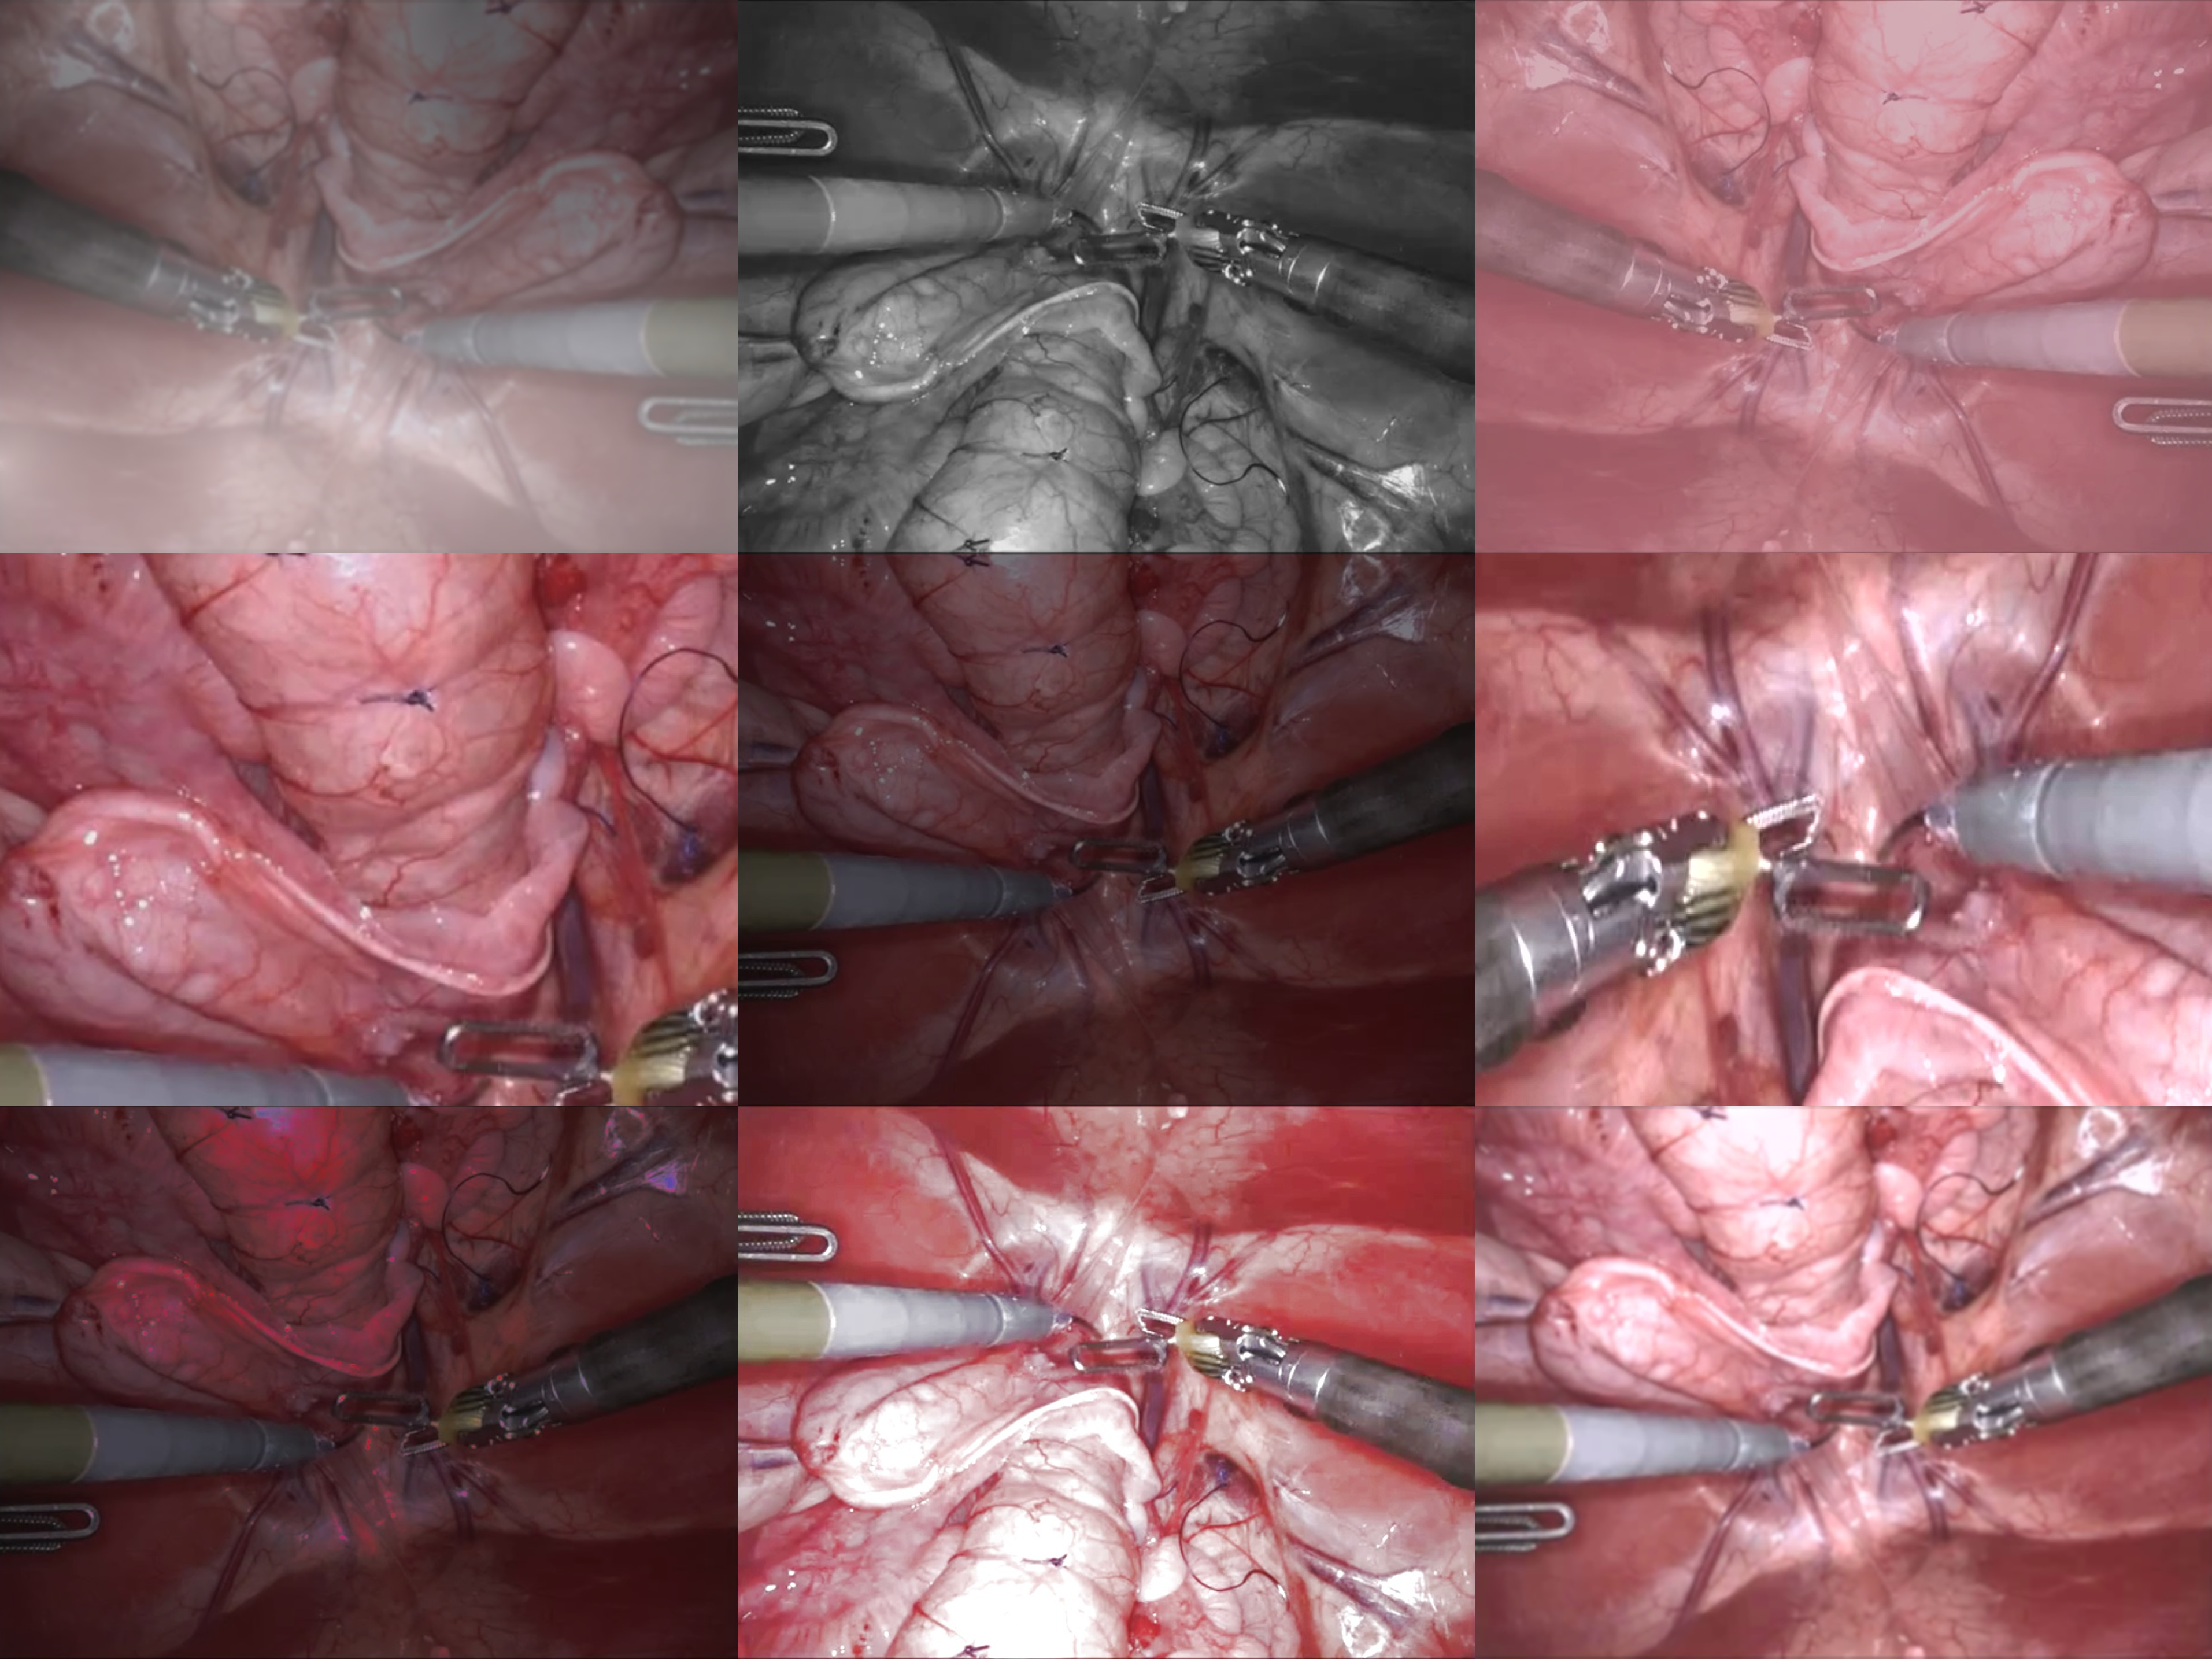
\includegraphics[width=0.8\textwidth]{img/compresspng/augmentations.png}
% 	\caption{Nine different sample variations of the same image from the DaVinci SurgVisDom dataset. Shown are random combinations of fog, grayscale, flip, blur, brightness, contrast and crop augmentations.} 	
% 	\label{in:fig:data_augmentation}
% \end{figure}

% As in \cite{detone2016deep}, we then crop the augmented image at edges $\{\mathbf{p}_i\}$, which we then deviate by $\{\Delta \mathbf{p}_i\}$. We apply the corresponding inverse homography to the full image and test whether all points $\{\mathbf{p}_i\}$ still reside within the polygon that is spanned by the new image edges. If so, we keep the sample $\{\mathbf{I}^\text{crop}_t, \mathbf{I}^\text{crop, warp}_{t+1}, \{\Delta\mathbf{p}_i\}\}$ as data point, else we resample $\{\Delta \mathbf{p}_i\}$. To regress $\{\Delta\mathbf{p}_i\}$ in between the sample $\{\mathbf{I}^\text{crop}_t, \mathbf{I}^\text{crop, warp}_{t+N}\}$, we further forward the image pair through a neural network and implement \eqref{in:eq:homography_linear} with the differentiable computer vision library Kornia \cite{riba2020kornia}. As DeTone et al. in \cite{detone2016deep}, we do this in a supervised manner, where we directly regress $\{\Delta\mathbf{p}_i\}$, however, as Nguyen et al. in \cite{nguyen2018unsupervised} and Zhang et al. in \cite{zhang2019content}, we further compute the loss in the image space on the tuple $\{\mathbf{I}^\text{crop}_t, \mathbf{I}^\text{crop, warp}_{t+N}\}$ in an unsupervised approach.
% \subsection{Experimental Setup}
% In our experimental setup, see \figref{in:fig:experimental_setup}, we use a  KUKA LBR Med 7 R800 robot. To control it, we create a bridge to ROS by wrapping the Fast Robot Interface (FRI) \cite{schreiber2010fast} with ROS' Hardware Interface functionality. We mount the laparoscope to the LBR Med 7 robot with a custom designed 3D print. As the laparoscope, we use a Storz 7230 AA Telescope, from which we capture images using a Storz TH 102 H3-Z FI Camera. For illumination, we additionally connect a Storz TL 300 Power LED 300 light source to the laparoscope. The acquired images are sent to the Storz TC 300 Image1 S H3-Link, which links the camera via DP to the Storz TC 200 Image1 S Connect. From there on, the image feed is output to SDI, which we convert to HDMI with a SDI to HDMI converter. We then grab the HDMI signal with a DeckLink 4K Extreme 12G and stream it onto the ROS network.

% \subsection{Data}
% To facilitate imitation learning on laparoscopic surgery data, we extract and isolate camera motion from object motion. Therefore, we collect DaVinci surgery data, where the camera only moves occasionally and is mostly fixed in position, but objects are still moving. We isolate data without camera motion from data with camera motion. We additionally collect laparoscopic surgery data with camera motion to imitate it. An exhaustive overview of publicly available datasets is given in \tabref{in:tab:datasets}. We analyze the data for its length, frame rate, resolution and camera motion. We pre-process the laparoscopic data by searching for its center point and bounding circle. We do so by seeking a circle who's radius and center fit best to the edge filtered laparoscopic view with a random sample consensus (RANSAC) \cite{fischler1981random}, see \figref{in:fig:ransac_circle}.

% \begin{figure}
% 	\centering
% 	\includegraphics[width=0.8\textwidth]{img/compresspng/ransac_0.png}
% 	\caption{RANSAC detection of the circular boundary of the laparoscopic image from Cholec80 \cite{twinanda2016endonet} (yellow). The turquoise rectangle is the maximum sized rectangle of a given aspect ratio that fits around the circle's center point. An example \href{https://drive.google.com/file/d/1aY7jnBoKNwKyMlSthjzgsRldkHEK1OKw/view?usp=sharing}{video} is provided.}
% 	\label{in:fig:ransac_circle}
% \end{figure}

% \begin{landscape}
% \begin{table}
% \centering
% \caption{Exhaustive overview of publicly available MIS datasets. All datasets were acquired and analyzed for task-appropriate metrics. in:tab:datasetsMetrics were marked with N/A, where datasets were not available or unreasonable to analyze.}
% \label{in:tab:datasets}
%     \begin{tabular}{|c|c|c|r|c|c|c|c|}
%         \hline
%         \multirow{2}{*}{Collection} & \multicolumn{7}{c|}{Specifications} \\
%         \cline{2-8}
%         & Name & Year & Length / \# & Frame Rate / Hz & Resolution / pixels & Camera Motion & Note \\
%         \hline
%         \multirow{8}{*}{\href{https://endovis.grand-challenge.org/}{\shortstack{Endoscopic\\Vision\\Challenge}}} &\href{https://www.synapse.org/#!Synapse:syn21776936/wiki/601700}{MISAW} \cite{mitsuishi2013master}&2020&$128102$&$30$&$460\times 540$&no&synthetic \\
%         \cline{2-8}
%         &\href{https://surgvisdom.grand-challenge.org/}{SurgVisDom}\cite{zia2021surgical}&2020&$185620$&$20$&$540\times960$&occasional&DaVinci \\
%         \cline{2-8}
%         &\href{https://robustmis2019.grand-challenge.org/}{ROBUST-MIS} \cite{maier2020heidelberg}\cite{ross2020robust}&2019&$7546968$&$25$&$540\times 960$&yes&laparoscopic \\
%         \cline{2-8}
%         &\href{https://endovissub2019-scared.grand-challenge.org/}{SCARED}&2019&$16818$&$25$&$1024 \times 1280$&yes& exoscopic \\
%         \cline{2-8}
%         &\href{https://endovissub-workflowandskill.grand-challenge.org/}{SWASA}&2019&N/A&N/A&N/A&yes& laparoscopic\\
%         \cline{2-8}
%         &\href{https://endovissub2017-workflow.grand-challenge.org/}{SWASA}&2018&N/A&N/A&N/A&yes& laparoscopic\\
%         \cline{2-8}
%         &\href{https://endovissub2018-roboticscenesegmentation.grand-challenge.org/home/}{RSS} \cite{allan20202018}&2018&$2235$&$2$&$1024\times 1280$&occasional& DaVinci\\
%         \cline{2-8}
%         &\href{https://endovissub2017-roboticinstrumentsegmentation.grand-challenge.org/}{RIS} \cite{allan20192017}&2017&$3225$&$2$&$1024\times 1280$&occasional& DaVinci \\
%         \cline{2-8}
%         &\href{https://endovissub2017-kidneyboundarydetection.grand-challenge.org/}{KBD}&2017&$3000$&$2$&$1024\times 1280$&occasional & DaVinci\\
%         \cline{2-8}
%         &\href{https://endovissub-instrument.grand-challenge.org/}{ISAT}&2015&$16243$&$25$&$480\times 640/576\times 720$& yes & laparoscopic \\
%         \hline
%         \multirow{3}{*}{\href{http://hamlyn.doc.ic.ac.uk/vision/}{\shortstack{Hamlyn\\Center\\Datasets}}} &\href{http://hamlyn.doc.ic.ac.uk/vision/data/daVinci.zip}{Siamese}\cite{ye2017self}&2017&$34240$&$30$&$192\times 384$& occasional& DaVinci \\
%         \cline{2-8}
%         &Giannarou \href{http://hamlyn.doc.ic.ac.uk/vision/data/Matina/Blur/capture1.avi}{left} / \href{http://hamlyn.doc.ic.ac.uk/vision/data/Matina/Blur/capture2.avi}{right} \cite{giannarou2012probabilistic}&2012&$8063$&$30$&$480\times 640$& occasional& DaVinci \\ 
%         \cline{2-8}
%         &Mountney \href{http://hamlyn.doc.ic.ac.uk/vision/data/Dataset8/left.avi}{left} / \href{http://hamlyn.doc.ic.ac.uk/vision/data/Dataset8/right.avi}{right} \cite{mountney2010three}&2010&$14418$&$30$&$480\times 640$& occasional & DaVinci\\
%         \hline
%         \multirow{4}{*}{Other} &\href{https://www.youtube.com/}{YouTube}&N/A&N/A&N/A&N/A&N/A & N/A \\
%         \cline{2-8}
%         &\href{https://saras-esad.grand-challenge.org/}{SARAS-ESAD} \cite{bawa2020esad}&2020&$18793$&$1$&$1080\times 1920$& occasional & DaVinci \\
%         \cline{2-8}
%         &\href{http://camma.u-strasbg.fr/datasets}{Cholec80} \cite{twinanda2016endonet}&2017&$4612530$&$25$&$480\times 854$&yes& laparoscopic\\
%         \cline{2-8}
%         &\href{https://cirl.lcsr.jhu.edu/research/hmm/datasets/jigsaws_release/}{JIGSAW} \cite{ahmidi2017dataset}&2016&$527491$&$30$&$480\times 640$&no& synthetic\\
%         \hline
%     \end{tabular}
% \end{table}
% \end{landscape}

% \section{RESULTS}
% In this section we first present and evaluate results for the visual servo in simulation in \secref{in:sec:results_visual_servo} and following that we analyze the homography regression performance in \secref{in:sec:results_homography_regression}. Finally, we measure the homography regression performance qualitatively in a dynamic surgical scene from a previously unseen dataset in \secref{in:sec:homography_imitation_learning}
% \subsection{Homography-based Visual Servo with RCM Objective}
% \label{in:sec:results_visual_servo}
% To demonstrate the effectiveness of the proposed visual servo, we implement an example, where the desired homography $\mathbf{H}$ is computed as a least squares solution with OpenCV's \textit{findHomography} function \cite{bradski2000opencv}. We extract key points from a calibration pattern, perturb the endoscope's position randomly and then iterate \eqref{in:eq:gain_controller} to minimize the task error $\mathbf{e}_\text{t}$ in \eqref{in:eq:error}, which is supposed to move the endoscope to the initial position. We set the task gain parameters $\mathbf{K}_\text{t} = \text{diag}(1.0,1.0,1.0,0.04,0.04,0.04)$ and the RCM gain parameters $\mathbf{K}_\text{RCM} = \text{diag}(100.0, 100.0, 100.0)$. We set the damping factor for the damped least squares inverse of the Jacobian matrix to $\gamma = 0.05$.
% An exemplary \href{https://drive.google.com/file/d/1xrPTe7FdxZiUFySA3CxLsW-lJGgMdrcS/view?usp=sharing}{video} is available on Google Drive. We evaluated the convergence of the task error $\mathbf{e}_\text{t}$, the deviation of the RCM $\mathbf{p}_\text{RCM}$ from the desired trocar position $\mathbf{p}_\text{trocar}$, as well as a visual error that we define as the mean pairwise distance of the key points found on the calibration board and the deviation of the tip position from the initial pose. Results are shown in \figref{in:fig:visual_servo_measurements}.

% \begin{figure}
% 	\centering
% 	\begin{subfigure}[b]{.4\textwidth}
% 		\centering
% 		\includegraphics[width=1.0\textwidth]{fig/task_error.pdf}
% 		\caption{Task error over time, refer to \eqref{in:eq:task}. The task, as computed from the desired homography, converges.}
% 	\end{subfigure}\hspace{2em}
% 	\begin{subfigure}[b]{.4\textwidth}
% 		\centering
% 		\includegraphics[width=1.0\textwidth]{fig/trocar_position_deviation.pdf}
% 		\caption{Trocar position deviation over time, refer to \eqref{in:eq:error}. The deviation stays below a couple of millimeters under task motion and converges again.}
% 	\end{subfigure}
% 	\begin{subfigure}[b]{.4\textwidth}
% 		\centering
% 		\includegraphics[width=1.0\textwidth]{fig/visual_error.pdf}
% 		\caption{The mean pairwise distance of calibration plane points in the normalized image plane converges.}
% 	\end{subfigure}\hspace{2em}
% 	\begin{subfigure}[b]{.4\textwidth}
% 		\centering
% 		\includegraphics[width=1.0\textwidth]{fig/tip_position_deviation.pdf}
% 		\caption{The tip position is first changed on purpose, then converges to close to zero after the visual servo is initialized but then starts to diverge, although the task errors are being minimized.}
% 	\end{subfigure}
% 	\caption{Evolution of different errors over time. In the setup, we perturb the laparoscope's tip and then initialize the homography-based visual servo to return to the initial position. Results were obtained in simulation.}
% 	\label{in:fig:visual_servo_measurements}
% \end{figure}

% \subsection{Homography Regression}
% \label{in:sec:results_homography_regression}
% As visualized in \figref{in:fig:datasets_sizes}, the datasets SurgVisDom, Giannarou and Mountney account for $72.4\%$ of data with occasional camera motion. 

% \begin{figure}
% 	\centering
% 	\begin{subfigure}[b]{.45\textwidth}
% 		\centering
% 		\includegraphics[width=1.\linewidth]{fig/fig_da_vinci.pdf}
% 		\caption{DaVinci surgery datasets modulo the Siamese dataset due to low resolution. The high frame rate datasets naturally cover $72.4\%$ of available data.}
% 		\label{in:fig:da_vinci}
% 	\end{subfigure}\hspace{2em}
% 	\begin{subfigure}[b]{.45\textwidth}
% 		\centering
% 		\includegraphics[width=1.\linewidth]{fig/fig_da_vinci_high_fps_laparoscopic.pdf}
% 		\caption{Laparoscopic datasets and a concatenation of the DaVinci high frame rate datasets. The ISAT dataset can barely be seen in this visualization. The Cholec80 dataset corresponds to about $51\,\text{h}$ of video.}
% 		\label{in:fig:da_vinci_laparoscopic}
% 	\end{subfigure}
% 	\caption{Dataset length visualizations for datasets listed in \tabref{in:tab:datasets}. Shown is the fraction of total number of images within a dataset.}
% 	\label{in:fig:datasets_sizes}
% \end{figure}

% $95\%$ of this data has no camera motion. We train all approaches from \secref{in:sec:implementation_homography_regression} on this data. We augment data with following probability
% \begin{itemize}
% 	\item Grayscale: $10\%$
% 	\item Horizontal flip: $50\%$
% 	\item Vertical flip: $50\%$
% 	\item Crop: $20\%$
% 	\item Brightness: $30\%$
% 	\item Gaussian blue: $10\%$
% 	\item Fog: $10\%$
% 	\item Contrast: $20\%$
% \end{itemize}
% Example augmentations are shown in \figref{in:fig:data_augmentation}. We train VGG-based networks and networks with a Resnet34 \cite{he2016deep} backbone. We use the Adam optimizer at a learning rate of $1\mathrm{e}{-4}$ and a momentum of $[0.9, 0.999]$. We set the batch size to $64$, the image crop shape to $480\times640$ and train for $20$ epochs on a train split with $80\%$ of the total data. The results are shown in \tabref{in:tab:train_results}. We excluded the results for the method from \cite{zhang2019content}, as it converged to the trivial solution.
% \begin{table}
% 	\centering
% 	\caption{Test loss on high frame rate DaVinci dataset without camera motion.}
% 	\begin{tabular}{ccc}
% 		Architecture & Supervised & Mean Pairwise Distance / pixels\\
% 		\hline
% 		VGG \cite{detone2016deep}         & yes & $4.547$ \\
% 		VGG \cite{nguyen2018unsupervised} & no  & $5.875$ \\
% 		Resnet34                          & yes & $\mathbf{1.566}$ \\
% 		Resnet34                          & no  & $2.944$	
% 	\end{tabular}
% 	\label{in:tab:train_results}
% \end{table}
% The Resnet34-backboned network performs the best.
% \subsection{Homography Imitation Learning}
% \label{in:sec:homography_imitation_learning}
% To qualitatively assess the homography estimation capability of the Resnet34-backboned network, we perform inference on the unseen Cholec80 dataset. We do so as the Cholec80 dataset accounts for about $37\%$ of available laparoscopic data, see \figref{in:fig:da_vinci_laparoscopic}, and consists of continuous video, whereas the ROBUST-MIS dataset only comprises short video clips of length $10\,\text{s}$. We compare the deep method against a SIFT feature-based homography estimation method. Exemplary alpha blends are shown in \figref{in:fig:alpha_blend}. Example videos of the alignment with \href{https://drive.google.com/file/d/1SpUtSVgwo_PAwAjULF-Ky_5CxRuhMYlm/view?usp=sharing}{stride 1} and \href{https://drive.google.com/file/d/17fmhSsPq290PuLXmtO-aWwo3KN4QkZA8/view?usp=sharing}{stride 10} are also provided on Google Drive.

% \begin{figure}
% 	\centering
% 	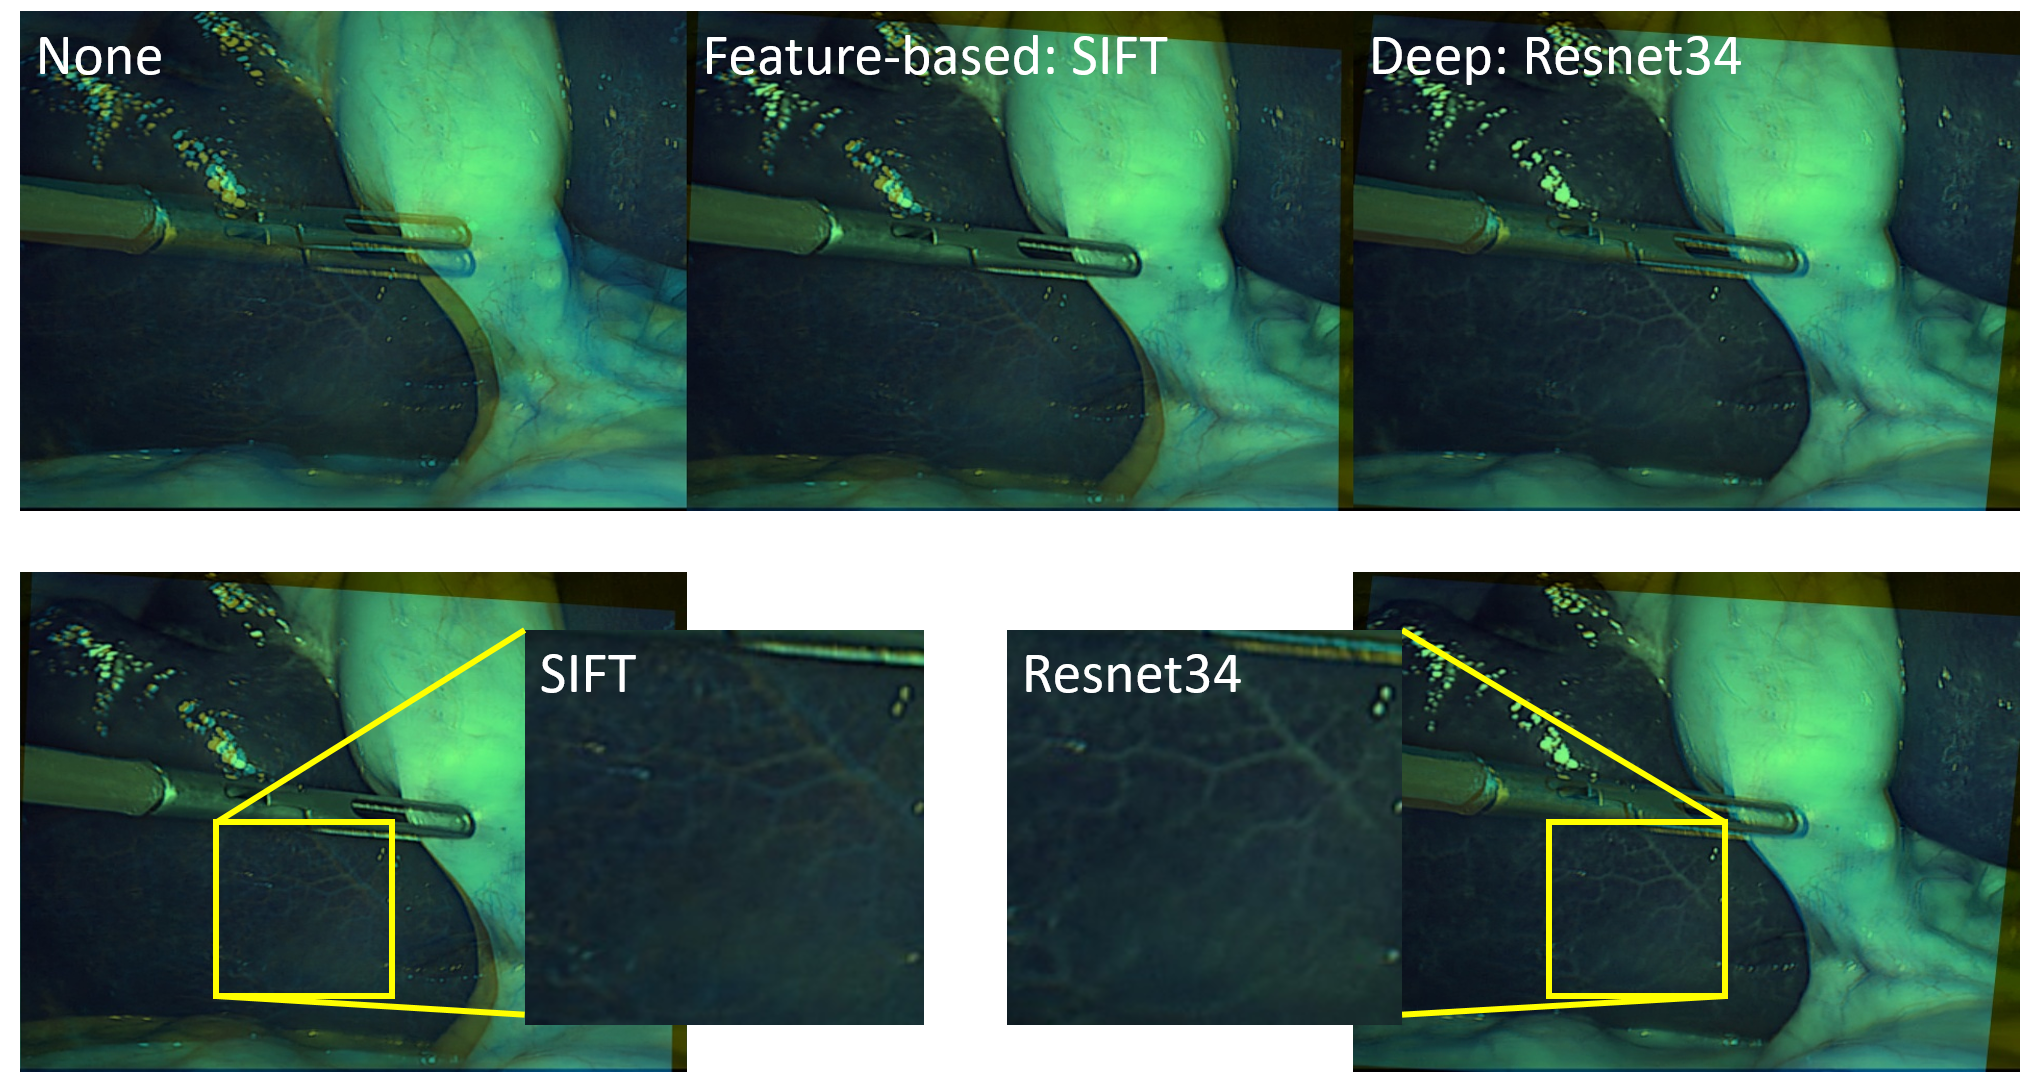
\includegraphics[width=.5\textwidth]{img/compresspng/blend_joint.png}
% 	\caption{Alpha blend of consecutive images from Cholec80 with stride $10$, corresponding to a $\Delta t$ of $0.4\,\text{s}$. Top row: The raw blend (none) shows severe camera and tool motion. The feature-based alignment breaks. The deep approach aligns both images well. Bottom row: The surgeon deforms the gallbladder while the camera is moving, the deep approach aligns the non-moving background well and ignores the deformation of the gallbladder, as can especially be seen in the zoom. Example videos of the alignment with \href{https://drive.google.com/file/d/1SpUtSVgwo_PAwAjULF-Ky_5CxRuhMYlm/view?usp=sharing}{stride 1} and \href{https://drive.google.com/file/d/17fmhSsPq290PuLXmtO-aWwo3KN4QkZA8/view?usp=sharing}{stride 10} are provided.}
% 	\label{in:fig:alpha_blend}
% \end{figure}

% Following the visual servo of \eqref{in:eq:twist}, we measure the severance of camera motion in a sequence of images by plotting the deviation of the estimated homography from the identity matrix against time, see \figref{in:fig:homography_annotation_moving_average}.

% \begin{figure}
% 	\centering
% 	\includegraphics[width=.5\textwidth]{fig/homography_annotation_moving_average.pdf}
% 	\caption{Moving average of L2-norm of homography matrix identity deviation, similar to \eqref{in:eq:twist}. The homography was regressed in between consecutive images with stride 1 from Cholec80 using a Resnet34 backbone. The chosen metric reveals uncontinuous camera motion, as can be seen through alternating minima and maxima. This aligns well with the visual observation from video.}
% 	\label{in:fig:homography_annotation_moving_average}
% \end{figure}

% \section{OUTLOOK}
% \subsection{Conclusion}
% In this work, we are the first to combine a homography-based visual servo task with a remote center of motion objective as an enabler for deep-learning based control in robotic laparoscopic surgery. We implement said controller as a ROS package for use on any robot and demonstrate its effectiveness in \secref{in:sec:results_visual_servo}. We observe task convergence but also tip position divergence, see \figref{in:fig:visual_servo_measurements}. This is caused by the homography extraction from a distant calibration pattern, which is unresponsive to change in distance. We then generate a new dataset of DaVinci surgeries from which we isolate camera motion. We train multiple deep homography regression approaches and list results in \tabref{in:tab:train_results}. We find that, other than proposed in \cite{detone2016deep}\cite{nguyen2018unsupervised}\cite{zhang2019content}, a Resnet34-backboned architecture performs the best. Based on this finding and on the dataset analysis in \figref{in:fig:da_vinci_laparoscopic}, we qualitatively evaluate the deep homography regression on the unseen dataset Cholec80 in \secref{in:sec:homography_imitation_learning}. We find central views within this data with a RANSAC method, see \figref{in:fig:ransac_circle}. We observe in \figref{in:fig:alpha_blend} that this method regresses camera motion well and isolates it from object motion. We also demonstrate the superiority over traditional SIFT feature-based homography estimation. Finally, we show in \figref{in:fig:homography_annotation_moving_average} that the homography regression can be used to reveal uncontinuous camera motion in video data, which aligns well with visual observation.
% \subsection{Shortcomings and Future Work}
% Although we demonstrate future potential for the presented approach, there are still shortcomings that are yet to be addressed. The results for the visual servo were taken from simulation, the toy calibration pattern homography extraction does not yet run on the real setup. The toy homography extraction also showed diverging properties for the tip of the laparoscope in simulation, which will be addressed by replacing the type homography extraction in the future. We further note that many of the homography regression results are not yet backed by quantitative measures. This will be accounted for by creating a human-labelled ground truth data subset. To now achieve an autonomous robotic endoscope, we will extend the work starting from \figref{in:fig:homography_annotation_moving_average}, where the potential of a next best view planning was revealed from the data at hand. We will further implement a force control on the real robot for feedback to extend the pipeline into an active learning approach.
